\documentclass{xduugthesis}
\usepackage[ruled,linesnumbered]{algorithm2e}
\xdusetup{
	style = {
		after-skip = {18pt,12pt,12pt,12pt,10pt,10pt},
		before-skip = {20pt,14pt,14pt,14pt,12pt,12pt},
	},
	info = {
		bib-resource={thesis.bib}
	}
}
\begin{document}
\chapter{概述}
\section{研究背景和意义}
合成孔径雷达(Synthetic Aperture Radar, SAR)是一种利用雷达信号的相位和幅度信息来生成图像的技术。它通过移动的雷达平台发射和接收信号,然后对这些信号进行处理,以产生高分辨率的图像。SAR技术在军事、地质勘探、环境监测、农业和城市规划等多个领域有着广泛的应用。\par
在实际应用中,尤其是对于遥感图像进行目标识别的情况下,使用者需要对大量的图像进行融合操作。在这个过程中,不同的图像融合方法都会对最终图像的效果产生不同的影响。在这个方面,本毕设将会调用实现一些常见的图像融合算法,并进行评估,从而加深对这些图像融合算法的认识。\par
同时,由于目前公开的合成孔径雷达数据集比较少,尤其缺少对一个目标点进行多角度成像的图片数据集。本毕设将会实现一个对雷达成像过程的仿真,并基于此进行包装,编写一个仿真生成合成孔径雷达图像特征图像程序。\par
最终,为了方便最终用户使用,我们需要将上述提到的融合算法和仿真程序进行包装,并进行用户界面包装,从而让用户更加直接地使用这些功能。\par
本合成孔径雷达图像融合程序可以使用户更加容易地进行雷达图像融合。同时,通过对图像融合算法的评估,用户可以更加直观地了解到这些算法的特点,从而挑选更加合适的算法,或者进一步优化。程序里面的仿真模块也是入门雷达图像扫描过程的直观参考。\par
\section{研究内容}
本毕设主要解决三个问题:针对合成孔径雷达图像特征进行图像融合,仿真生成合成孔径雷达图像特征的图像,根据用户界面优化成为一个程序。\par
在针对合成孔径雷达图像特征进行图像融合方面,本毕设需要在了解图像分解和融合原理的基础上,引用和实现一些常见的图像分解融合方法。同时,我们需要在了解图像评估方法对基础上,对各个方法融合的图像进行评估。\par
在仿真生成合成孔径雷达图像特征的图像方面,本毕设需要寻找合适的工具,进行对合成孔径雷达扫描目标点,形成图像过程的模拟。进而,获得对一个目标点进行多角度的图像,方便用户在没有数据的情况下,使用这个软件,进而对合成孔径雷达成像和图像融合结果形成一个初步的认知。\par
最后,在根据用户界面优化成为一个程序方面,我们需要将这些功能的交互进行优化,从而使用户更直观地使用本程序。
\section{论文结构}
本论文共分为五章,具体结构如下:\par
第一章是概述。主要是为了提出本毕设需要解决的问题,以及本毕设一个大致的架构。\par
第二章介绍了相关技术。本章主要介绍本毕设所涉及的主要背景,包括雷达简介,图像融合技术和仿真使用的软件。\par
第三章介绍了系统的设计和实现。根据第一章提到的毕设大致架构,阐述了本毕设的实现方法和细节,以及如何让用户更加方便地使用本软件。\par
第四章介绍了本软件运行的状况。本章模拟了两个用户使用场景,展示了本软件使用指南,同时展示了图像融合算法的处理结果。\par
第五章对文章进行总结和展望,总结所做的工作并给出未来的研究方向和展望。
\chapter{相关技术背景}
\section{合成孔径雷达}
本段将会对合成孔径雷达进行简单介绍,同时介绍其成像步骤。
\subsection{简介}
合成孔径雷达(英语:synthetic aperture radar, SAR)\cite{SAR_Introduction},属于一种微波成像雷达,也是一种可以产生高分辨率图像的(航空)机载雷达或(太空)星载雷达。它通过移动的雷达平台发射和接收电磁波信号,然后对这些信号进行处理,以产生高分辨率的图像。使用SAR雷达成像,相比使用光学设备,能够穿透云层和雾层笼罩,进而较不受天气影响。与此同时,由于利用了电磁波反射的特性,SAR雷达成像能够体现出地貌或被观测物体的特征。目前,该技术在军对地观测、行星观测、目标定位、无人驾驶等领域中有着广泛的应用。\par
根据种类,合成孔径雷达可以形成可以分成单发单收、单发多收等系统。这些是根据在一个雷达系统中,发出信号的设备和接收设备的多少来进行分类的。在目标定位中,使用多个信号源能够提高成像的信号量,从而提高定位精度。本论文只讨论单发单收的状况。
\subsection{成像过程}
根据刘国祥的介绍\cite{SAR_Process},我在此简要描述单发单收合成孔径雷达的成像过程。\par
\begin{figure}[h!]
	\centering
	\includegraphics[scale=0.25]{img/sar.jpg}
	\caption{合成孔径雷达成像过程图示例}
\end{figure}
我们假设雷达的天线宽度是W,长度是L。雷达按照轨道,在高度H上运行。雷达以一个侧视角$\theta_0$发射一个椭圆锥状的微波脉冲,该脉冲垂直于轨道飞行方向。其垂直于轨道的顶角称为波束高度角$\omega_v$,它与雷达天线宽度是W和雷达波长$\lambda$相关,即:
$$\omega_v=\frac{\lambda}{W}$$
其沿轨的椭圆锥顶角$\omega_h$则与雷达天线长度L相关,即:\par
$$\omega_h=\frac{\lambda}{L}$$
该微波脉冲将会在地面形成一个辐照带。由上可知,雷达天线越宽,辐射带照得越远;天线越长,辐射带照得越宽。\par
辐照带的辐宽是垂直于轨道方向的辐照带长度,计算方式如下:\par
$$W_G\approx\frac{{\lambda}R_m}{wcos\eta}$$
其中,$R_m$为雷达中心到辐照带中心的斜距,$\eta$为该中心点的雷达入射角。\par
评估SAR雷达成像的信息量和效果称为分辨率,也就是可以区分两个相邻目标的最小距离。分辨率越小越好。分辨率有两个方向的,称为方位角分辨率$\Delta X$和斜距向分辨率$\Delta R$。\par
其中,方位向分辨率(azimuth range)是沿雷达飞行方向的分辨率,按照雷达斜距R和雷达长度确定,计算公式为:\par
$$\Delta\ X=R\omega_h=\frac{R\lambda}{L}$$
斜距向分辨率(slant range)是垂直于雷达飞行方向的分辨率,而当其投射到地面时候,是斜距向地面分辨率$\Delta Y$。这两个分辨率和光速c,脉冲宽度$\tau_p$和侧视角$\theta_i$相关,计算公式为:\par
$$\Delta R=\frac{c\tau_p}{2}$$
$$\Delta Y=\frac{\Delta R}{cos(90^\circ-\theta_i)}=\frac{c\tau_p}{2cos(90^\circ-\theta_i)}$$
下图展示了SAR雷达的一次扫描形成的辐照带和分辨率。\par
在实际应用中,我们需要针对一个目标点不停成像,从而提高目标的分辨率。斜距向分辨率的参数只和雷达性能参数相关,改善的话不能从此着手。我们需要利用多普勒频移现象来改善雷达成像的方位向分辨率。假设长度为L的雷达天线从a移动到b再到c(其中b为ac之间的中点),在扫描目标过程中,我们需要测定脉冲的延迟,跟踪频率转移。最后合成一个脉冲,提高目标成像分辨率。此时方位向分辨率$\Delta X$可以近似表述为:\par
$$\Delta X=\frac{L}{2}$$
\subsection{成像特征}
上述得到的回波数据,需要通过方位向和斜距向压缩才能获得原始数据。由此获得的雷达成像数据,每一个像素包含了亮度值和相对雷达飞行方向的斜距上有关的相位值,存储的是复数信息\cite{SAR_Pixel},即:
$$Pixel\rightarrow a+b \cdot i$$
像素的亮度值是由该像素振幅决定的,其计算方式为该像素复数的模长,即$\sqrt{a^2+b^2}$。振幅越大,表示地表反射强度越大。该像素相位值计算方式为$\varphi = \tan^{-1}(\frac{b}{a})$。因此,合成孔径雷达图像又称复数图像。\par
像素的亮度值由雷达特性、测试角度,表面朝向和粗糙度决定。比如,平静的湖面等十分平坦的表面,在雷达灰度上呈现全黑,而城市等比较粗糙的表面就为亮区域。\par
像素的相位值是该像素点上所有散射体分布决定的,而波的散射必然是带有方向的,故而产生了相位。在实际成像中,由于散射体的随机分布,造成了产生的强度和相位随像素的不同而变化,分别呈现指数分布和均匀分布。
\begin{figure}[h!]
	\centering
	\includegraphics[scale=0.25]{img/sar_image_pixel.jpg}
	\caption{像素的表示形式,可见是散射体随机分布的累加}
\end{figure}

\subsection{波段种类}
无论是什么雷达,发射的都是电磁波。根据上文对分辨率的描述,电磁波的波长会影响方位向分辨率。以下是常用的雷达波长列表\cite{SAR_Radar_Wavelenngth}:
\begin{table}[h!]
	\begin{center}
		\caption{雷达常用波长列表}
		\begin{tabular}{|c|c|c|}
			\hline
			\textbf{波长名称} & \textbf{波长范围} & \textbf{备注}\\
			\hline
			$L$ & 1 GHz 到 2 GHz & 长波 \\
			\hline
			$S$ & 2 GHz 到 4 GHz & 短波 \\
			\hline
			$C$ & 4 GHz 到 8 GHz & S 波和 X 波的过渡 \\
			\hline
			$X$ & 8 GHz 到 12 GHz &  \\
			\hline
			$K_u$ & 12 GHz 到 18 GHz & 小于 K 波 \\
			\hline
			$K$ & 18 GHz 到 27 GHz &  \\
			\hline
			$K_a$ & 27 GHz 到 40 GHz & 大于 K 波 \\
			\hline
		\end{tabular}
	\end{center}
\end{table}

\section{图像融合算法}
本段介绍图像融合算法的大致步骤,本毕设涉及的图像融合算法。
\subsection{原理和意义}
图像融合过程是指从多幅图像中收集所有重要信息,并将其合并成较少的图像,通常是单幅图像。这种单一图像比任何单一来源的图像信息量更大、更准确,而且包含所有必要的信息。图像融合的目的不仅在于减少数据量,还在于构建更适合人类和机器感知、更易于理解的图像。图像融合过程分为图片分解方法和图像融合方法,而最终的算法是由一个分解方法和一个合成方法组成的。\par
在本毕设中,我们需要将多张对单个目标多角度扫描所形成对一系列图像进行合成,最后形成一张最大程度包括这些成像信息的图像,提高该图像的信息量。
\subsection{图像分解方法}
图像分解方法是对同一个目标一系列图像的特征进行分解,从而获取出图像的一系列特征。以下介绍常见的图像分解算法。\par
\begin{enumerate}
\item \textbf{小波图像分解方法}\cite{Wavelet_Merge}基于一个限制时域的,会衰减的小波基来对图像进行处理。小波可以进行在时间上的拉伸和收缩过程,以及在信号延迟上的提前和错后。小波变换相比经常使用的傅立叶变换,能够知道各个成分出现的时间,知道信号频率随时间变化的情况。这个应用到图像,可以做到让图像每个频谱的时空信息都能保留,并能对其进行分析。在本毕设中,我将使用haar小波来进行小波变换。\par
下图展示了对图像使用小波算法分解后,会得到图像的低频信息,水平方向的高频信息,垂直方向的高频信息和对角线的高频信息。同时,我们可以对低频信息继续分解,进行多次图像分解。\par
\begin{figure}[h!]
	\centering
	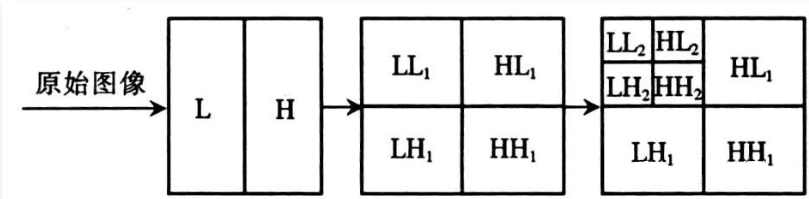
\includegraphics[scale=0.2]{img/wavelet.png}
	\caption{本图表示了一次小波分解的过程}
\end{figure}
小波图像分解融合算法实现在很多重要的图形处理库都有,比如OpenCV,MATLAB的图像处理包等。\par
接下来四张图像分别表示一张图片一次小波分解后的低频信息,水平方向、竖直方向和对角线方向的高频信息。\par
\begin{figure}[h!]
	\centering
	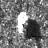
\includegraphics[scale=1.5]{img/wavelet-a.jpg}
	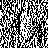
\includegraphics[scale=1.5]{img/wavelet-h.jpg}
	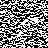
\includegraphics[scale=1.5]{img/wavelet-v.jpg}
	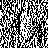
\includegraphics[scale=1.5]{img/wavelet-d.jpg}
	\caption{从左到右表示图像一次小波分解的低频,水平、垂直、对角线高频的信息}
\end{figure}
\item \textbf{NSCT图像分解方法}\cite{NSCT_Merge}是在小波分解的基础上,基于金字塔分解滤波器和非下采样方向滤波器,对图像进行高低频和方向面的分解。首先,使用金字塔分解滤波器多次分解图像,得到低频和高频信息。然后,对分解后的高频分量进行方向分解,分解成为不同方向上的细节信息。\par
NSCT图像分解方法相比小波图像分解方法,可以更加精细地分解图像,更好地保留出高频信息(比如图像中的线,边缘等信息),同时避免了信号变化极大的时候容易出现的振荡现象。\par
NSCT图像处理算法成熟的实现目前只有随该分解方法论文附带的MATLAB处理库\cite{NSCT_MATLAB}。下图展示其分解后的状况:\par
\begin{figure}[h!]
	\centering
	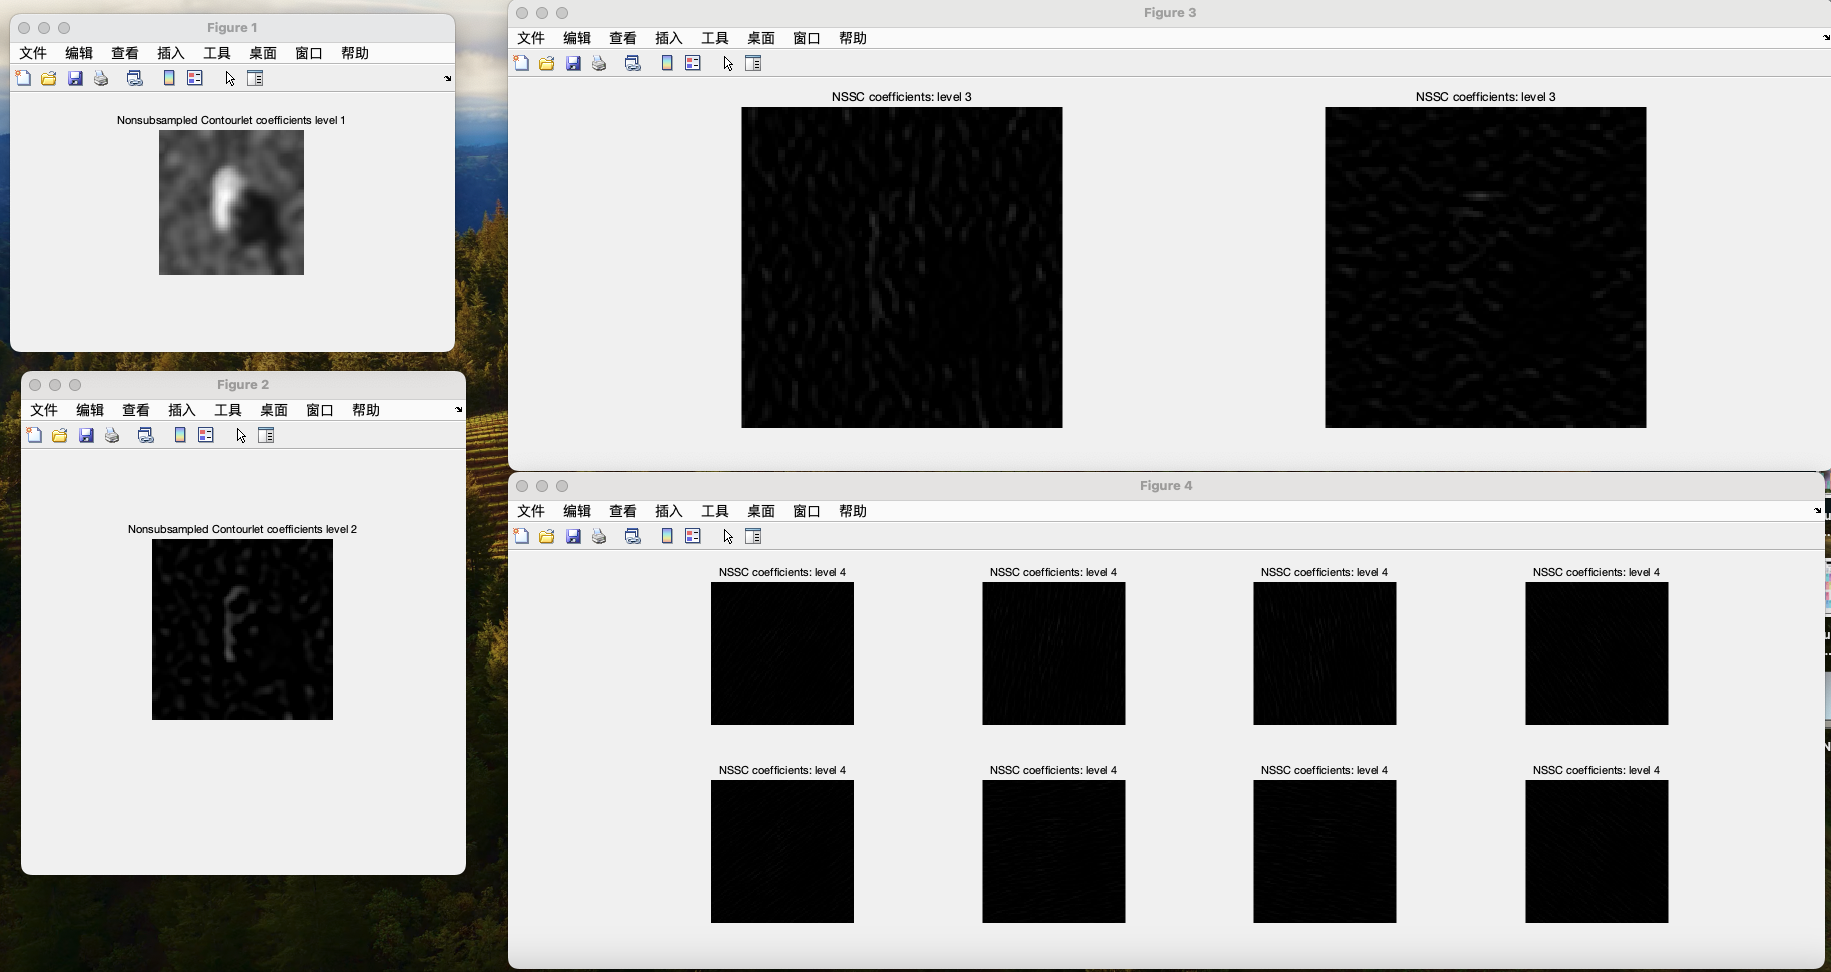
\includegraphics[scale=0.2]{img/nsct_result.png}
	\caption{NSCT 三次分解示例,左上角是低频信息,左下角是一次分解的高频信息,右上角表示两次分解的高频信息,右下角表示三次分解的高频信息}
\end{figure}

\end{enumerate}
\subsection{图像融合方法}
图像融合方法是针对上述提到分解成果,选择适当的方式提取图像特征,进而进行融合。最后,进行上述图像分解方法的逆向方法,最后成为一张融合后的图像。\par
\begin{enumerate}
\item \textbf{最大绝对值融合法}是逐像素来进行融合的方法。目标是将每个图像中,最突出的信息集中到最终融合图像中,从而,提高最终图像的信息量。像素信息的突出方式,也就是该像素的亮度,在黑白影像中,一般按照八位的无符号整数来表示。\par
本方法需要对每张需要融合图片的同一位置像素亮度进行分析,以绝对值最大者为最终融合图像对应位置的的像素。公式如下:
$$w_{dk}^{i,j}=max\left(\{\left|w_{dn}^{i,j}\right|,n\in\left[1,K\right],n\in N^\ast\}\right)$$
其中,$K$表示输入的图像数量。
其算法实现为:\par
\IncMargin{1em}
\begin{algorithm}
	\SetKwData{Left}{left}\SetKwData{This}{this}\SetKwData{Up}{up}
	\SetKwFunction{Union}{Union}\SetKwFunction{FindCompress}{FindCompress}
	\KwData{一系列相同大小的图片矩阵$Im$,大小是$w\times l$,数量是$length$}
	\KwResult{融合后的图片矩阵$I$}
	将$I$设置为$w\times l$的全0矩阵\;
	\For{$i\leftarrow w$}{
		\For{$j\leftarrow l$}{
			$value\_array \leftarrow$长度为$length$的数组\;
			\For{$pic\leftarrow length$}{
				$value\_array[pic] \leftarrow Im[pic][i][j]$的绝对值\;
			}
			$I[i][j] \leftarrow value\_array$中的最大值\;
		}
	}
	\caption{最大绝对值融合法}
\end{algorithm}
\DecMargin{1em}
\item \textbf{主成分变换融合法}是基于主成分变换这一数学统计过程,结合小波变换低频信息而得出的图像合成算法。\par
主成分变换(principal component analysis, PCA)是一个常用的数据降维算法,通过这个算法,可以提取出数据的特征。\par
根据这篇论文\cite{PCA_Merge},我们可以将分解方法生成的低频信息进行主成分变换,然后将第一个分量作为新的近似图像。之后,将近似低频信号和高频信号分别按照以下公式进行加权:
$$HH(x,y)=\sum_{i=1}^{N}k_iHH_i(x,y)$$
$$k_i=\mu_i/\sum_{i=1}^{N}\mu_i$$
其中,$\mu_i$表示第$i$个图像的数据平均值,$HH_i(x,y)$表示需要融合的第$i$个图像,$HH(x,y)$表示融合后的图像。
其算法实现为:\par
\IncMargin{1em}
\begin{algorithm}
	\SetKwData{Left}{left}\SetKwData{This}{this}\SetKwData{Up}{up}
	\SetKwFunction{Union}{Union}\SetKwFunction{FindCompress}{FindCompress}
	
	\KwData{一系列相同大小的图片矩阵$Im$,大小是$w\times l$,数量是$length$}
	\KwResult{融合后的图片矩阵$I$}
	使用一次图像分解算法,分解图片$Im$\;
	$Ilow\leftarrow$ 分解图片后的低频信息,数量是$length$\;
	$Ihigh\leftarrow$ 分解图片后的高频信息,数量随分解算法而不同\;
	$Inewlow\leftarrow$ 融合后的低频信息\;
	$Inewhigh\leftarrow$ 融合后的高频信息\;
	$value\_array\leftarrow$ 长度为$length$的数组\;
	\For{$It\leftarrow Ilow, Ihigh$}{
		\If(低频信息进行主成分变换或得权重){${It}=={Ilow}$}{
			\For{$i\leftarrow length$}{
				$pca\_level \leftarrow$ $Ilow[i]$ 长宽高的最小值 $ * 0.75$\;
				$Ilow[i] \leftarrow$ 对 $Ilow[i]$ 进行 $pca\_level$ 层主成分变换的结果\;
				$value\_array\leftarrow Ilow[i]$ 所有值的平均值\;
			}
			$value\_array \leftarrow value\_array / value\_array$ 的总和\;
			\For{$j\leftarrow length$}{
				$Inewlow\leftarrow Ilow[j] * value\_array[j]$\;
			}		
		}
		\For{$j\leftarrow length$}{
			$Inewhigh\leftarrow Ihigh[j] * value\_array[j]$\;
		}
	}
	对 $Inewlow$ 和 $Inewhight$ 进行逆变换\;
	\caption{主成分变换融合法}
\end{algorithm}
\DecMargin{1em}
\item \textbf{核范式加权融合法}是基于核范式这一矩阵信息,结合小波变换低频信息而得出的图像合成算法。\par
图像的核范式,是其我们可以通过对图像进行SVD奇异值分解,然后通过累加矩阵奇异值,获得核范式。\par
本方法需要对每张图片的奇异值进行分析,然后整体进行权重加权融合,得出最终融合的图像。该方法的权重公式\cite{Softmax_Merge}如下:
$$w_{dk}^{i,j}=\frac{w_{dk}^{\hat{i},j}}{\sum_{q=1}^{K}w_{dq}^{\hat{i},j}}$$
$$w_{dk}^{\hat{i},j}={\left\| re\left(V_{dk}^{i,j}\right)\right\|}_*$$
其中,$re\left(V_{dk}^{i,j}\right)$表示需要重构的图像,$\cdot_*$表示该图像的核范式,$K$表示输入的图像数量。\par
其算法实现为:\par
\IncMargin{1em}
\begin{algorithm}
	\SetKwData{Left}{left}\SetKwData{This}{this}\SetKwData{Up}{up}
	\SetKwFunction{Union}{Union}\SetKwFunction{FindCompress}{FindCompress}
	\KwData{一系列相同大小的图片矩阵$Im$,大小是$w\times l$,数量是$length$}
	\KwResult{融合后的图片矩阵$I$}
	将$I$设置为$w\times l$的全0矩阵\;
	$value\_array\leftarrow$ 长度为$length$的数组\;
	\For{$i\leftarrow length$}{
		$value\_array \leftarrow Im[i]$经过SVD分解后获得的奇异值\;
	}
	$value\_array \leftarrow value\_array / value\_array$ 的总和\;
	\For{$j\leftarrow length$}{
		$Inewlow\leftarrow Ilow[j] * value\_array[j]$\;
	}		
	\caption{核范式加权融合法}
\end{algorithm}
\DecMargin{1em}
\end{enumerate}
\subsection{融合结果评估指标}
对于融合后的图像,只凭人肉眼的主观判断是不够的,使用一些参数进行量化评估是很有必要的。以下介绍一些常用的图像信息量化评估方法\cite{Eval}:\par
\begin{enumerate}
\item 图片的\textbf{熵值}(entropy)代表了图片所包含的信息量。具体定义为:
$$EN=-\sum_{i=0}^{L-1}p_ilog_2p_i$$
其中$L$代表灰度级数,$p_i$代表图片灰度级的直方图。其值越大,表示图片包含的信息越多。\par
\item 图片的\textbf{标准差}(standard deviation, SD)表示图片信息的离散程度,其公式如下:
$$SD=\sqrt{\sum_{i=1}^{M}\sum_{j=1}^{N}(F(i,j)-\mu)^2}$$
其中$\mu$表示图片的均值。其值越大,表示数据离散程度越高,图片越能突出表示特征。
\item 融合后的图片和融合前图片的\textbf{互信息},表示融合前后图像信息的相关性,该值越大越能表示相关性越强。
\item 图片的\textbf{空间频率}(spatial frequency,SF) 是通过测量融合图像的梯度分布,揭示融合图像的细节和纹理信息的指标。具体定义为
$$SF = RF^2 + CF^2$$
式中, $RF = \sqrt{\sum_{i=1}^{M}\sum_{j=1}^{N}(F(i,j)-F(i,j-1))^2}$表示行频率。\par
$CF = \sqrt{\sum_{i=1}^{M}\sum_{j=1}^{N}(F(i,j)-F(i-1,j))^2}$表示列频率。\par
更高的空间频率意味着更加丰富的边缘和纹理细节。
\end{enumerate}
\section{MATLAB程序环境}
本段介绍本毕设涉及到的MATLAB以及雷达仿真工具箱。
\subsection{MATLAB}
MATLAB(Matrix Laboratory,矩阵实验室)是由美国 The MathWorks 公司出品的商业数学软件。
它是一种用于算法开发、数据可视化、数据分析以及数值计算的高级技术计算语言和交互式环境。除了常见的矩阵运算和绘制函数/数据图像等功能外,MATLAB还可以用来创建用户界面,调用其他语言(包括C、C++、Java、Python、FORTRAN)编写的程序。主要用于数值运算,但利用众多附加工具箱,它也适用于不同领域的应用,例如控制系统设计与分析、影像处理、深度学习、信号处理与通讯、金融建模和分析等。此外,配套软件包Simulink提供可视化开发环境,常用于系统模拟、动态/嵌入式系统开发等方面。截至2020年,全球有超过400万用户使用MATLAB,涵盖工程、科学和经济学等领域。
\subsection{MATLAB雷达仿真工具箱}
MATLAB雷达仿真工具是在2021年由美国MathWorks公司发布的雷达仿真工具,其中包括了设计、仿真、分析和测试多功能雷达系统的算法和工具。通过该工具,用户可以设计、模拟、分析和测试多功能雷达系统,进而加速项目的验证和落地。\par
目前,该工具在汽车雷达仿真、合成孔径雷达仿真、以及机载雷达设计方面得到了广泛应用。
\chapter{系统设计与实现}
\section{图像融合模块}
这里介绍本毕设中,图像融合模块的实现。本模块本质上是一系列图像融合算法的MATLAB实现,它们是综合了第二章提到的图像融合算法而实现的。同时,我还将使用MSTAR数据来融合图片,然后对结果进行评估,从而评价这些融合算法。\par
需要注意的是,无论本毕设的结果如何,这些算法都将集成到最终的图像融合软件中,提供给用户使用。
\subsection{融合算法实现}
通过对图像融合方法的分析和比较,我将实现以下算法:
\begin{enumerate}
\item \textbf{一次小波分解,最大绝对值融合法}\par
小波变换作为最广泛使用的图像分解算法,我将其作为分解图片的参照组。同时,最大绝对值融合法的编程和运算相对简单,于是将其作为融合时候的参照组。\par
本方法步骤如下:
\begin{enumerate}
	\item 对于输入的一系列图片,各进行一次小波分解。得到图片的低频信息和水平方向、竖直方向和对角线方向的高频信息。
	\item 对于每一个分解信息,进行最大绝对值融合法图像融合。
	\item 对于融合后的信息,使用小波变换的逆变换,完成融合步骤。
\end{enumerate}
\item \textbf{一次小波分解,主成分变换融合法}\par
这个方法是参考2.2.3.2方法实现的。由于小波多层分解中,下一层的分解利用了上一次分解的低频信息,如果输入图片过小,则造成多层分解后,最底层的低频信息主成分过少,从而没必要进行降低主成分操作。所以,本方法仅会进行一次小波分解。\par
本方法步骤如下:
\begin{enumerate}
	\item 对于输入的一系列图片,各进行一次小波分解。得到图片的低频信息和水平方向、竖直方向和对角线方向的高频信息。
	\item 对于图片的低频,使用主成分变换法,获取其第一个主成分分量。然后,分别计算这些信息的平均值,从而获得融合权重。
	\item 根据权重,对于每层图片的每一个分解信息,根据上一个步骤的权重进行加权平均融合。
	\item 对于融合后的信息,使用小波变换的逆变换,完成融合步骤。
\end{enumerate}
\item \textbf{三次小波分解,最大绝对值融合法}\par
如上个方法所述,小波变换的下一层分解是基于上一次分解的低频信息。所以,如果我们能多层进行分解,并在每层进行融合,也许会对融合后图像的质量提升有很大帮助。\par
本方法步骤如下:
\begin{enumerate}
	\item 对于输入的一系列图片,各进行三次小波分解。得到图片的低频信息和高频信息。
	\item 对于分解后的信息,使用最大绝对值融合法进行融合。
	\item 对于融合后的信息,从底层到高层,使用小波变换的逆变换,完成融合步骤。
\end{enumerate}
\item \textbf{三次小波分解,核范式加权融合法}\par
在上一个方法的基础上,对数据量较大的低频信息使用核范式加权法,对数据量较低的高频信息使用绝对值最大法,进而集中数据。\par
本方法步骤如下:
\begin{enumerate}
	\item 对于输入的一系列图片,各进行三次小波分解。得到图片的低频信息和高频信息。
	\item 对于分解后的信息,低频信息使用核范式加权法,高频使用最大绝对值融合法进行融合。
	\item 对于融合后的信息,从底层到高层,使用小波变换的逆变换,完成融合步骤。
\end{enumerate}
\item \textbf{一次NSCT分解,最大绝对值融合法}\par
这个方法使用NSCT金字塔式分解,用于和纯小波变换进行比较。本方法步骤如下:
\begin{enumerate}
	\item 对于输入的一系列图片,各进行一次NSCT分解。得到图片的低频信息和高频信息。
	\item 对于分解后的信息,低频使用核范式加权融合法进行融合,对于高频信息,使用最大绝对值融合法进行融合。
	\item 对于融合后的信息,从底层到高层,使用小波变换的逆变换,完成融合步骤。
\end{enumerate}
\item \textbf{三次NSCT分解,主成分变换融合法}\par
NSCT的层级分解其只会生成一个低频信息,因为它的层级分解是针对高频信息的。所以,我们可以对NSCT三次分解,然后都使用主成分融合法进行加权融合。\par
本方法步骤如下:
\begin{enumerate}
	\item 对于输入的一系列图片,各进行三次NSCT分解。得到图片的低频信息和高频信息。
	\item 对于分解后的低频信息,使用主成分变换法,获取其第一个主成分分量。然后,计算这些信息的平均值,获得融合权重。
	\item 使用融合权重进行分解后信息的加权融合。
	\item 对于融合后的信息,使用NSCT变换的逆变换,完成融合步骤。
\end{enumerate}
\item \textbf{三次NSCT分解,核范式加权融合法}\par
对应三次小波变换和核范式加权融合法,加上NSCT分解出来的高频信息更少,高频用最大值融合法更能集中信息。\par
本方法步骤如下:
\begin{enumerate}
	\item 对于输入的一系列图片,各进行三次NSCT分解。得到图片的低频信息和三层高频信息。
	\item 对于分解后的信息,低频信息使用核范式加权融合法,各层高频信息使用最大绝对值融合法。
	\item 对于融合后的信息,从底层到高层使用三次NSCT变换的逆变换,完成融合步骤。
\end{enumerate}
\end{enumerate}
\subsection{评估融合算法}
这里将会使用五张来自MSTAR数据集的坦克当作测试数据,这些数据都附带了角度,方便不用对准直接融合。图片的预处理步骤如下:
\begin{enumerate}
	\item 按照图片附带的角度,将图像进行旋转,使目标位于图像中央。
	\item 裁剪图片,去除因旋转产生的黑边。
\end{enumerate}
\begin{figure}[h!]
	\centering
	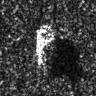
\includegraphics[scale=0.8]{img/1-cropped.jpg}
	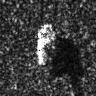
\includegraphics[scale=0.8]{img/2-cropped.jpg}
	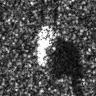
\includegraphics[scale=0.8]{img/3-cropped.jpg}
	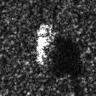
\includegraphics[scale=0.8]{img/4-cropped.jpg}
	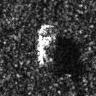
\includegraphics[scale=0.8]{img/5-cropped.jpg}
	\caption{需要融合的图像实例,图片已经经过旋转裁剪处理}
\end{figure}\par
在预处理后,使用算法融合图像,然后对其熵值、标准差、空间频率,和对原先照片相比较得出的互信息中位数进行评估。
\begin{figure}[h!]
	\centering
	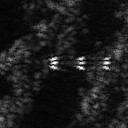
\includegraphics[scale=0.8]{img/result_straight.jpg}
	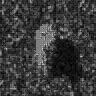
\includegraphics[scale=0.8]{img/result_wavelet_pca.jpg}
	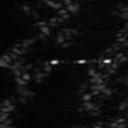
\includegraphics[scale=0.8]{img/result_wavelet.jpg}
	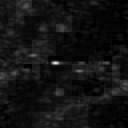
\includegraphics[scale=0.8]{img/result_wavelet_softmax.jpg}\par
	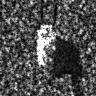
\includegraphics[scale=0.8]{img/result_nsct.jpg}
	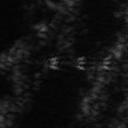
\includegraphics[scale=0.8]{img/result_nsct_pca.jpg}
	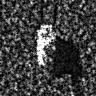
\includegraphics[scale=0.8]{img/result_nsct_softmax.jpg}
	\caption{融合结果,从左到右代表对照组中的一次小波分解,最大绝对值融合法;一次小波分解,主成分变换融合法;三次小波分解,最大绝对值融合法;三次小波分解,核范式加权融合法;一次NSCT分解,最大绝对值融合法;三次NSCT分解,主成分变换融合法;三次NSCT分解,核范式加权平均法}
\end{figure}
\begin{table}[h!]
	\begin{tabular}{|c|c|c|c|c|}
		\hline
		融合方式 & 图片熵值 & 标准差 & 空间频率 & 互信息中位数 \\
		\hline
		一次小波分解,最大绝对值融合法 & 7.4593 & 52.8821 & 13.9746 & 1.9261  \\
		\hline
		一次小波分解,主成分变换融合法 & 6.4928 & 24.7216 & 9.1857 & 1.5282  \\
		\hline
		三次小波分解,最大绝对值融合法 & 7.0148 & 43.9587 & 12.6562 & 1.6993 \\
		\hline
		三次小波分解,核范式加权融合法 & 7.0204 & 43.7315 & 12.6518 & 1.7007  \\
		\hline
		三次nsct分解,最大绝对值融合法 & 7.4049 & 53.1878 & 13.6282 & 1.9373 \\
		\hline
		三次nsct分解,主成分变换融合法 & 6.7062 & 37.0415 & 10.3018 & 1.6980 \\
		\hline
		三次nsct分解,核范式加权融合法 & 7.2330 & 51.8677 & 13.5779 & 1.8665 \\
		\hline
	\end{tabular}
	\caption{融合结果评估指标一览}
\end{table}\par
根据这些信息,以及肉眼观察,可以简要总结这五个融合算法:
\begin{enumerate}
	\item 在图像分解方面,同样的分解层数下,使用 NSCT 方法能比小波融合保留更多的信息量,同时,也能保留更多图片共同的信息。同时,对于小波分解,多层分解对于保留图像整体信息是很有必要的。
	\item 对于主成分变换融合法,该方法是步骤最复杂,融合效果也是最差的。不仅是肉眼上图片的模糊现象明显,而且在一系列指标方面都显著低于平均水平。
	\item 对于绝对值最大法,虽然能够体现相对更好的评估指标,但是在肉眼呈现上,信息有所损失。尤其是针对目标最上面的一处阴影,大多数使用该方法融合的图片,都没能体现。因此,小波变换和绝对值最大法结合的融合方法会导致信息的损失。但是,该方法可以集中信息量,这会对一些信息量相对较少的信息有很好的融合效果。
	\item 对于核范式权重法,该方法能够更好地体现图像之间的权重信息。尤其是在后三个方法上,不仅在指标上都有优势,而且在肉眼上,该方法的图片能够保留更多的信息。而该融合方法与NSCT方法的结合,能够在指标上和完全的绝对值最大法相媲美。
\end{enumerate}

\section{仿真获取数据模块}
本模块用于描述本程序仿真SAR雷达扫描的步骤,以及对数据的处理。目标是对雷达运行过程中,对一个目标点从多角度成像过程进行模拟。本段大幅参考MATLAB官方示例\cite{SAR_Simulation}。
\subsection{该过程的必要性}
本毕设需要对地面上的目标点进行多角度扫描后的图像数据。而在这个方面,目前关于SAR雷达成像数据比较少,其中最著名的是欧洲的ERS-1数据\cite{ERS}和美国军方的MSTAR数据\cite{MSTAR}。欧洲的ERS-1数据是很清晰的遥测数据,但是,这些数据缺少对一个目标多角度的扫描成图,而只是将图片旋转后裁剪,和显示成像结果。而MSTAR虽然包含了对一个目标多角度的扫描,但是目标过小,不利于图像的融合。因此,自行生成多角度的扫描图对于本毕设很有必要。\par
【插入点这俩玩意图片】\par
目前开源的合成孔径雷达软件只有RaySAR\cite{RaySAR}用户比较多,但是这个软件用途是分析建筑物结构的。虽然使用了合成孔径雷达模拟,但是不符合本毕设的用途。最后,本毕设决定使用MATLAB提供的雷达工具箱来进行仿真。
\subsection{随机地形生成}
随机地形生成是利用系统随机数,在三维度x-y-z坐标轴上面,生成用于模拟扫描成像的地形信息。地形包括位置,大小和海拔。\par
在生成地形的时候,我们需要考虑以下信息:
\begin{enumerate}
	\item 地形在坐标轴上的位置,需要输入在三维坐标轴上,X轴的范围和Y轴的范围。
	\item 初始高度和最高海拔数据。
	\item 迭代次数,迭代次数越多,地面越平滑,但是过多迭代次数会导致地面过于平坦。
	\item 粗糙值,该值越小,生成的地形越粗糙,该值越大,生成的地形越平滑。默认设为 2。
\end{enumerate}
模拟步骤如下:
\begin{enumerate}
	\item 根据输入的坐标轴范围,获取变化率,生成地形生成范围。
	\item 根据初始高度,平均海拔数据和之前设置的高度数据(如果不是第一次),生成固定大小的高度信息。
	\item 将海拔小于0的部分设为0。
	\item 根据设置的迭代次数,重复第2步和第3步。
	\item 将高度信息放缩到地形生成范围内,返回坐标轴和高度信息。
\end{enumerate}\par
在本次模拟中,本毕设将在X轴$[900, 1600]$范围,Y轴$[-400, 400]$范围内生成地形。其粗糙值为1.5,最高海拔100,初始海拔0度。生成过程中,需要循环8次。\par
在生成随机地形之后,需要设置该地形上面的信号反射率。本仿真中,高于40的地形设为丘陵森林,小于40的设为森林。
\subsection{目标点放置}
目标点的放置是为了方便我们对仿真成像结果进行分辨,为此,需要在合适的位置和高度放置目标点。放置步骤如下:\par
\begin{enumerate}
	\item 初始化一个三列矩阵,分别代表三维度x-y-z坐标轴的坐标值。然后,将坐标数据填入其中,高度设为0。
	\item 使用坐标轴找到地形上的对应位置,然后设定高度。这样就结束了目标点的放置。
\end{enumerate}
在本毕设仿真中,目标点将会放在$(1000,0)$为中心的位置m这个位置将会是仿真的中心位置。
\subsection{模拟雷达参数}
考虑到软件使用平台的运转速度,以及模拟成像的分辨率,在本人多次尝试后,决定仿真数据基于L波段雷达,参数如下:
\begin{table}[h!]
	\begin{center}
		\caption{仿真雷达数据}
		\begin{tabular}{|c|c|}
			\hline
			波长 & 1 GHz \\
			\hline
			信号带宽 & 30 MHz \\
			\hline
			脉冲宽度 & 0.003 ms  \\
			\hline
			采样频率 & 60 MHz \\
			\hline
			脉冲重复频率 & 500 \\
			\hline
		\end{tabular}
	\end{center}
\end{table}\par
该参数代表了一个L波长的合成孔径雷达,其方位向的分辨率大致为5米。在接下来的模拟中,该雷达将会在距离地面1000米的高度运行。
\subsection{雷达运动轨迹}
本毕设参考了由该篇论文\cite{SAR_Observation_Model}所提到的SAR雷达协作监测模型,同时根据本毕设的需求,设计了本毕设中雷达的路径。\par
首先,我们需要知道成像的中心点。根据3.2.2节的描述,中心点在$(1000,0)$的位置。同时,根据数据推算的辐照带大小,我们将在距离目标点x-y平面上1000米位置成像,同时,考虑到雷达运行的高度,雷达天线角度大致为45度。与此同时,考虑到SAR雷达的侧视和成像大小,我们需要让雷达按照100米每秒的速度运行两秒时间。\par
同时,由于本次模拟涉及到对一个目标点进行多角度的成像,这里需要用户输入成像时候的角度。\par
综上所述,本毕设的路径中点将在以$(1000,0)$为中心的圆上。其路径也将与该圆半径相切,长度为400米。同时,规定$(0,0)$为0度的成像路径中点。路径示例如下:
【描述根据目标点】
【绘制图画】
在路径方面,涉及到路径的动态运算。所以,需要用户提供成像角度,然后计算目标点的起始点和结束点。其路径计算算法如下:\par
\IncMargin{1em}
\begin{algorithm}
	\SetKwData{Left}{left}\SetKwData{This}{this}\SetKwData{Up}{up}
	\SetKwFunction{Union}{Union}\SetKwFunction{FindCompress}{FindCompress}
	
	\KwData{成像的角度$\theta$,路径中点$(x_0,y_0)$,旋转参考点$(x,y)$,雷达运行速度$v$,运行时间$dur$}
	\KwResult{路径的起点$(x_{start},y_{start})$和终点$(x_{end},y_{end})$}
	\tcp{计算路程中点}
	$x_{mid} \leftarrow x + (x_0 - x) * cos(\theta) - (y_0 - y) * sin(\theta)$\;
	$y_{mid} \leftarrow y + (y_0 - y) * cos(\theta) + (x_0 - x) * sin(\theta)$\;
	\tcp{通过中点计算起点}
	$x_{start} \leftarrow x_{mid} + \frac{v * dur * sin(angle)}{2} $\;
	$y_{start} \leftarrow y_{mid} + \frac{v * dur * cos(angle)}{2} $\;
	\tcp{计算雷达在X轴和Y轴上面的速度}
	$v_x \leftarrow v * sin(\theta)$\;
	$v_y \leftarrow v * cos(\theta)$\;
	\tcp{通过速度计算终点}
	$x_{stop} \leftarrow x_{start} + v_x * dur $\;
	$y_{stop} \leftarrow y_{start} + y_x * dur $\;
	\caption{路径起点终点计算}
\end{algorithm}
\DecMargin{1em}

以下是程序运行过程中,所展示的路径概览。\par
【程序图片截图】
\subsection{模拟流程}
\begin{enumerate}
	\item 初始化地形,设置放射率,放置目标点。
	\item 使用radarScenario函数设置雷达仿真环境,同时将地形数据和目标点数据放置在platform结构体里,然后放在仿真环境中。
	\item 使用rdr数组初始化雷达信息,将雷达放置在仿真环境中。
	\item 计算雷达位置和目标点位置的夹角,将其作为雷达天线夹角。
	\item 根据用户输入的角度,设置雷达的路径,然后进行成像数据仿真获取。
	\item 使用rangeMigrationLFM函数对数据进行处理,得到形成单视复合(SLC)图像数据。
\end{enumerate}
\subsection{数据保存}
通过上述仿真得到的成像结果,是一个复数矩阵。复数的模长能够描述该点的信号强度,所以,我们需要将该矩阵转换为以模长为数据的矩阵。\par
在此之后,根据上文提到的运行轨迹和分辨率,我们需要对图片进行大小调整,使其能够反应地貌和目标点状态。这些参数是根据雷达的波长,采样频率,以及运行轨迹决定的。算法如下:
\IncMargin{1em}
\begin{algorithm}
	\SetKwData{Left}{left}\SetKwData{This}{this}\SetKwData{Up}{up}
	\SetKwFunction{Union}{Union}\SetKwFunction{FindCompress}{FindCompress}
	\KwData{图像矩阵$slcimg$, 最小采样率$minSample$, 雷达运行速度$v$, 采样频率$fs$, 脉冲重复频率$prf$}
	\KwResult{放缩后的图片矩阵$I$}
	\tcp{根据方位向分辨率计算图片高度}
	$numPulses \leftarrow slcimg$ 的高度 \tcp*{获取采集到的脉冲}
	$du \leftarrow v/prf $\tcp*{脉冲间距}
	$dky \leftarrow 2\pi /numPulses*du $\tcp*{在对应波长下的间距}
	$dy \leftarrow 2\pi / numPulses*dky $\tcp*{一个脉冲代表的长度}
	$y \leftarrow dy * numPulses$ \;
	\tcp{根据斜距向分辨率计算图片长度}
	$numSamples \leftarrow slcimg$ 的高度 \tcp*{获取采集样点数量}
	$samples \leftarrow [minSample, minSample + numSamples - 1] $\tcp*{获取采样范围}
	$sampleTime \leftarrow samples / fs $\tcp*{采样时间}
	$rngVec \leftarrow $通过光速和采样时间获取长度范围\;
	$x \leftarrow max(rngVec) - min(rngVec)$\;
	\tcp{处理图像矩阵}
	$img \leftarrow abs(slcimg)$ 然后转置\;
	$img \leftarrow $将图片 $img$ 按照长 $x$ 宽 $y$ 的设定重新放缩\;
	\caption{图片后期放缩方法}
\end{algorithm}
\DecMargin{1em}

【简介雷达数据】
【方向分辨率和速度分辨率的描述】
【成像一览】
\section{终端输入设计}
\subsection{选择图片}
\subsection{输入角度}
\subsection{进度条显示}
\chapter{运行展示}
\section{用户输入模式}
\section{仿真运行模式}

\chapter{总结和展望}

\end{document}